\documentclass{standalone}
\usepackage{tikz}
\usetikzlibrary{patterns}
\usetikzlibrary{positioning}
\usetikzlibrary{patterns, positioning}
\usetikzlibrary{shapes.misc}
\usepackage[outline]{contour}
\contourlength{1.5pt} 


\begin{document}
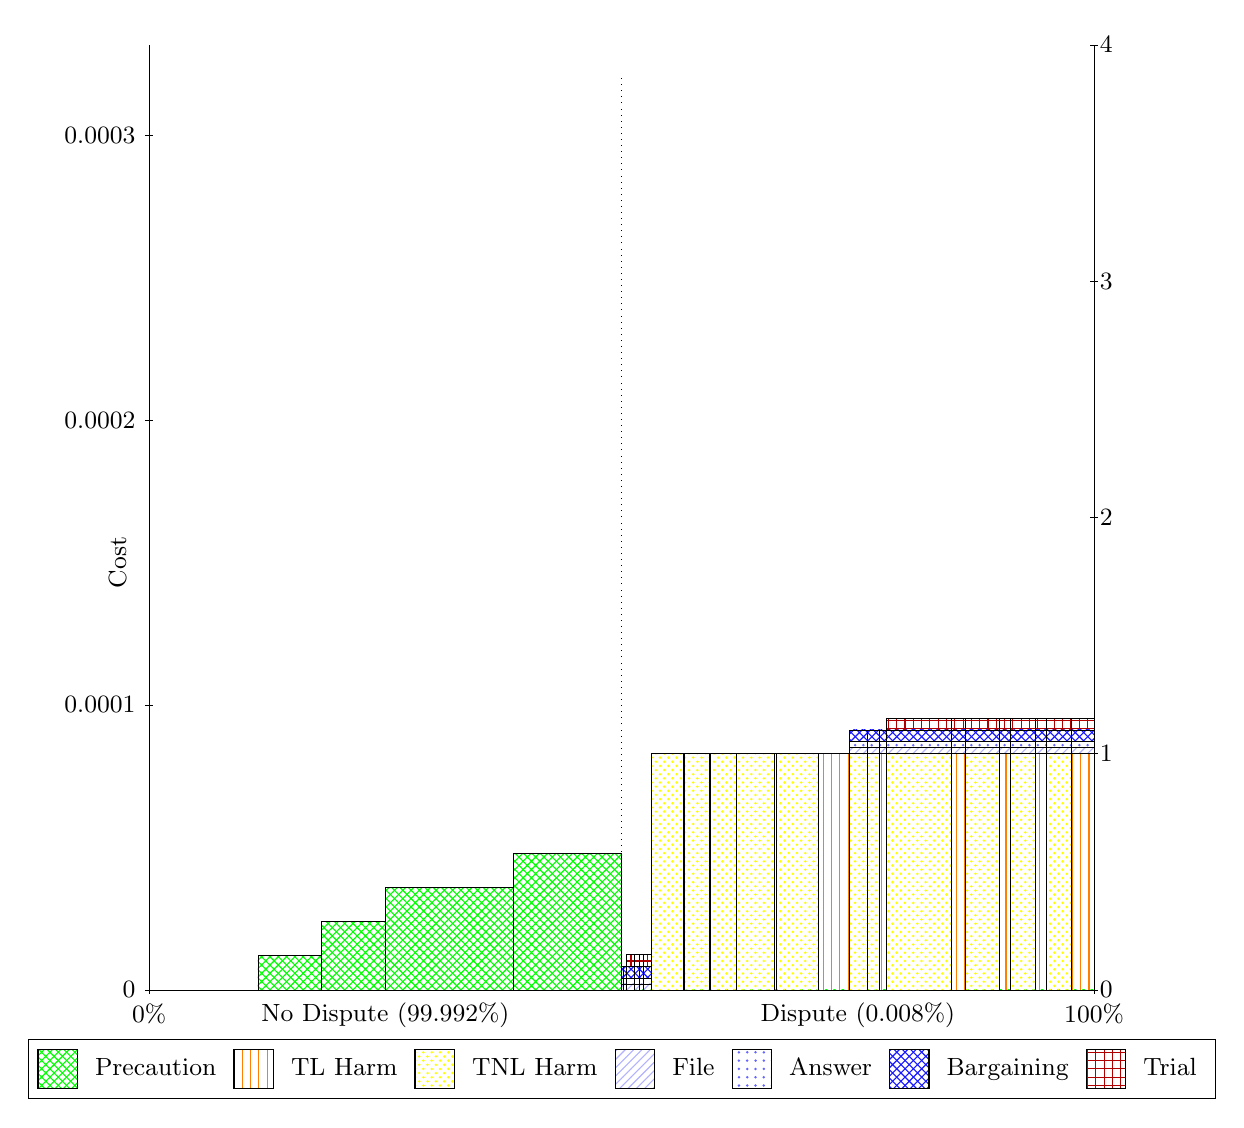
\begin{tikzpicture}
\draw[pattern=crosshatch, pattern color=green,draw=black,very thin] (2.8801,2.5) rectangle (3.6907,2.9341);
\draw[pattern=crosshatch, pattern color=green,draw=black,very thin] (3.6907,2.5) rectangle (4.5,3.3682);
\draw[pattern=crosshatch, pattern color=green,draw=black,very thin] (4.5,2.5) rectangle (6.1199,3.8023);
\draw[pattern=crosshatch, pattern color=green,draw=black,very thin] (6.1199,2.5) rectangle (7.5,4.2363);
\draw[pattern=north east lines, pattern color=blue!30,draw=black,very thin] (7.5,2.5) rectangle (7.5233,2.575);
\draw[pattern=dots,  pattern color=blue!60,draw=black,very thin] (7.5,2.575) rectangle (7.5233,2.65);
\draw[pattern=crosshatch,      pattern color=blue!90,draw=black,very thin] (7.5,2.65) rectangle (7.5233,2.8);
\draw[pattern=crosshatch, pattern color=green,draw=black,very thin] (7.5233,2.5) rectangle (7.558,2.5001);
\draw[pattern=north east lines, pattern color=blue!30,draw=black,very thin] (7.5233,2.5001) rectangle (7.558,2.5751);
\draw[pattern=dots,  pattern color=blue!60,draw=black,very thin] (7.5233,2.5751) rectangle (7.558,2.6501);
\draw[pattern=crosshatch,      pattern color=blue!90,draw=black,very thin] (7.5233,2.6501) rectangle (7.558,2.8001);
\draw[pattern=north east lines, pattern color=blue!30,draw=black,very thin] (7.558,2.5) rectangle (7.659,2.575);
\draw[pattern=dots,  pattern color=blue!60,draw=black,very thin] (7.558,2.575) rectangle (7.659,2.65);
\draw[pattern=crosshatch,      pattern color=blue!90,draw=black,very thin] (7.558,2.65) rectangle (7.659,2.8);
\draw[pattern=grid,            pattern color=red!70!black,draw=black,very thin] (7.558,2.8) rectangle (7.659,2.95);
\draw[pattern=crosshatch, pattern color=green,draw=black,very thin] (7.659,2.5) rectangle (7.7209,2.5);
\draw[pattern=north east lines, pattern color=blue!30,draw=black,very thin] (7.659,2.5) rectangle (7.7209,2.575);
\draw[pattern=dots,  pattern color=blue!60,draw=black,very thin] (7.659,2.575) rectangle (7.7209,2.65);
\draw[pattern=crosshatch,      pattern color=blue!90,draw=black,very thin] (7.659,2.65) rectangle (7.7209,2.8);
\draw[pattern=grid,            pattern color=red!70!black,draw=black,very thin] (7.659,2.8) rectangle (7.7209,2.95);
\draw[pattern=crosshatch, pattern color=green,draw=black,very thin] (7.7209,2.5) rectangle (7.7785,2.5001);
\draw[pattern=north east lines, pattern color=blue!30,draw=black,very thin] (7.7209,2.5001) rectangle (7.7785,2.5751);
\draw[pattern=dots,  pattern color=blue!60,draw=black,very thin] (7.7209,2.5751) rectangle (7.7785,2.6501);
\draw[pattern=crosshatch,      pattern color=blue!90,draw=black,very thin] (7.7209,2.6501) rectangle (7.7785,2.8001);
\draw[pattern=grid,            pattern color=red!70!black,draw=black,very thin] (7.7209,2.8001) rectangle (7.7785,2.9501);
\draw[pattern=crosshatch, pattern color=green,draw=black,very thin] (7.7785,2.5) rectangle (7.8696,2.5001);
\draw[pattern=north east lines, pattern color=blue!30,draw=black,very thin] (7.7785,2.5001) rectangle (7.8696,2.5751);
\draw[pattern=dots,  pattern color=blue!60,draw=black,very thin] (7.7785,2.5751) rectangle (7.8696,2.6501);
\draw[pattern=crosshatch,      pattern color=blue!90,draw=black,very thin] (7.7785,2.6501) rectangle (7.8696,2.8001);
\draw[pattern=grid,            pattern color=red!70!black,draw=black,very thin] (7.7785,2.8001) rectangle (7.8696,2.9501);
\draw[pattern=crosshatch dots, pattern color=yellow,draw=black,very thin] (7.8696,2.5) rectangle (8.2864,5.5);
\draw[pattern=vertical lines, pattern color=orange,draw=black,very thin] (8.2864,2.5) rectangle (8.2919,5.5);
\draw[pattern=crosshatch, pattern color=green,draw=black,very thin] (8.2919,2.5) rectangle (8.6185,2.5);
\draw[pattern=crosshatch dots, pattern color=yellow,draw=black,very thin] (8.2919,2.5) rectangle (8.6185,5.5);
\draw[pattern=crosshatch, pattern color=green,draw=black,very thin] (8.6185,2.5) rectangle (8.6231,2.5);
\draw[pattern=vertical lines, pattern color=orange,draw=black,very thin] (8.6185,2.5) rectangle (8.6231,5.5);
\draw[pattern=crosshatch, pattern color=green,draw=black,very thin] (8.6231,2.5) rectangle (8.953,2.5001);
\draw[pattern=crosshatch dots, pattern color=yellow,draw=black,very thin] (8.6231,2.5001) rectangle (8.953,5.5001);
\draw[pattern=crosshatch, pattern color=green,draw=black,very thin] (8.953,2.5) rectangle (8.9583,2.5001);
\draw[pattern=vertical lines, pattern color=orange,draw=black,very thin] (8.953,2.5001) rectangle (8.9583,5.5001);
\draw[pattern=crosshatch, pattern color=green,draw=black,very thin] (8.9583,2.5) rectangle (9.438,2.5001);
\draw[pattern=crosshatch dots, pattern color=yellow,draw=black,very thin] (8.9583,2.5001) rectangle (9.438,5.5001);
\draw[pattern=crosshatch, pattern color=green,draw=black,very thin] (9.438,2.5) rectangle (9.465,2.5001);
\draw[pattern=vertical lines, pattern color=orange,draw=black,very thin] (9.438,2.5001) rectangle (9.465,5.5001);
\draw[pattern=crosshatch, pattern color=green,draw=black,very thin] (9.465,2.5) rectangle (10.002,2.5001);
\draw[pattern=crosshatch dots, pattern color=yellow,draw=black,very thin] (9.465,2.5001) rectangle (10.002,5.5001);
\draw[pattern=crosshatch, pattern color=green,draw=black,very thin] (10.002,2.5) rectangle (10.392,2.5001);
\draw[pattern=vertical lines, pattern color=orange,draw=black,very thin] (10.002,2.5001) rectangle (10.392,5.5001);
\draw[pattern=crosshatch dots, pattern color=yellow,draw=black,very thin] (10.392,2.5) rectangle (10.613,5.5);
\draw[pattern=north east lines, pattern color=blue!30,draw=black,very thin] (10.392,5.5) rectangle (10.613,5.575);
\draw[pattern=dots,  pattern color=blue!60,draw=black,very thin] (10.392,5.575) rectangle (10.613,5.65);
\draw[pattern=crosshatch,      pattern color=blue!90,draw=black,very thin] (10.392,5.65) rectangle (10.613,5.8);
\draw[pattern=vertical lines, pattern color=orange,draw=black,very thin] (10.613,2.5) rectangle (10.624,5.5);
\draw[pattern=north east lines, pattern color=blue!30,draw=black,very thin] (10.613,5.5) rectangle (10.624,5.575);
\draw[pattern=dots,  pattern color=blue!60,draw=black,very thin] (10.613,5.575) rectangle (10.624,5.65);
\draw[pattern=crosshatch,      pattern color=blue!90,draw=black,very thin] (10.613,5.65) rectangle (10.624,5.8);
\draw[pattern=crosshatch, pattern color=green,draw=black,very thin] (10.624,2.5) rectangle (10.771,2.5001);
\draw[pattern=crosshatch dots, pattern color=yellow,draw=black,very thin] (10.624,2.5001) rectangle (10.771,5.5001);
\draw[pattern=north east lines, pattern color=blue!30,draw=black,very thin] (10.624,5.5001) rectangle (10.771,5.5751);
\draw[pattern=dots,  pattern color=blue!60,draw=black,very thin] (10.624,5.5751) rectangle (10.771,5.6501);
\draw[pattern=crosshatch,      pattern color=blue!90,draw=black,very thin] (10.624,5.6501) rectangle (10.771,5.8001);
\draw[pattern=crosshatch, pattern color=green,draw=black,very thin] (10.771,2.5) rectangle (10.859,2.5001);
\draw[pattern=vertical lines, pattern color=orange,draw=black,very thin] (10.771,2.5001) rectangle (10.859,5.5001);
\draw[pattern=north east lines, pattern color=blue!30,draw=black,very thin] (10.771,5.5001) rectangle (10.859,5.5751);
\draw[pattern=dots,  pattern color=blue!60,draw=black,very thin] (10.771,5.5751) rectangle (10.859,5.6501);
\draw[pattern=crosshatch,      pattern color=blue!90,draw=black,very thin] (10.771,5.6501) rectangle (10.859,5.8001);
\draw[pattern=crosshatch dots, pattern color=yellow,draw=black,very thin] (10.859,2.5) rectangle (11.69,5.5);
\draw[pattern=north east lines, pattern color=blue!30,draw=black,very thin] (10.859,5.5) rectangle (11.69,5.575);
\draw[pattern=dots,  pattern color=blue!60,draw=black,very thin] (10.859,5.575) rectangle (11.69,5.65);
\draw[pattern=crosshatch,      pattern color=blue!90,draw=black,very thin] (10.859,5.65) rectangle (11.69,5.8);
\draw[pattern=grid,            pattern color=red!70!black,draw=black,very thin] (10.859,5.8) rectangle (11.69,5.95);
\draw[pattern=vertical lines, pattern color=orange,draw=black,very thin] (11.69,2.5) rectangle (11.868,5.5);
\draw[pattern=north east lines, pattern color=blue!30,draw=black,very thin] (11.69,5.5) rectangle (11.868,5.575);
\draw[pattern=dots,  pattern color=blue!60,draw=black,very thin] (11.69,5.575) rectangle (11.868,5.65);
\draw[pattern=crosshatch,      pattern color=blue!90,draw=black,very thin] (11.69,5.65) rectangle (11.868,5.8);
\draw[pattern=grid,            pattern color=red!70!black,draw=black,very thin] (11.69,5.8) rectangle (11.868,5.95);
\draw[pattern=crosshatch, pattern color=green,draw=black,very thin] (11.868,2.5) rectangle (12.294,2.5);
\draw[pattern=crosshatch dots, pattern color=yellow,draw=black,very thin] (11.868,2.5) rectangle (12.294,5.5);
\draw[pattern=north east lines, pattern color=blue!30,draw=black,very thin] (11.868,5.5) rectangle (12.294,5.575);
\draw[pattern=dots,  pattern color=blue!60,draw=black,very thin] (11.868,5.575) rectangle (12.294,5.65);
\draw[pattern=crosshatch,      pattern color=blue!90,draw=black,very thin] (11.868,5.65) rectangle (12.294,5.8);
\draw[pattern=grid,            pattern color=red!70!black,draw=black,very thin] (11.868,5.8) rectangle (12.294,5.95);
\draw[pattern=crosshatch, pattern color=green,draw=black,very thin] (12.294,2.5) rectangle (12.43,2.5);
\draw[pattern=vertical lines, pattern color=orange,draw=black,very thin] (12.294,2.5) rectangle (12.43,5.5);
\draw[pattern=north east lines, pattern color=blue!30,draw=black,very thin] (12.294,5.5) rectangle (12.43,5.575);
\draw[pattern=dots,  pattern color=blue!60,draw=black,very thin] (12.294,5.575) rectangle (12.43,5.65);
\draw[pattern=crosshatch,      pattern color=blue!90,draw=black,very thin] (12.294,5.65) rectangle (12.43,5.8);
\draw[pattern=grid,            pattern color=red!70!black,draw=black,very thin] (12.294,5.8) rectangle (12.43,5.95);
\draw[pattern=crosshatch, pattern color=green,draw=black,very thin] (12.43,2.5) rectangle (12.758,2.5001);
\draw[pattern=crosshatch dots, pattern color=yellow,draw=black,very thin] (12.43,2.5001) rectangle (12.758,5.5001);
\draw[pattern=north east lines, pattern color=blue!30,draw=black,very thin] (12.43,5.5001) rectangle (12.758,5.5751);
\draw[pattern=dots,  pattern color=blue!60,draw=black,very thin] (12.43,5.5751) rectangle (12.758,5.6501);
\draw[pattern=crosshatch,      pattern color=blue!90,draw=black,very thin] (12.43,5.6501) rectangle (12.758,5.8001);
\draw[pattern=grid,            pattern color=red!70!black,draw=black,very thin] (12.43,5.8001) rectangle (12.758,5.9501);
\draw[pattern=crosshatch, pattern color=green,draw=black,very thin] (12.758,2.5) rectangle (12.891,2.5001);
\draw[pattern=vertical lines, pattern color=orange,draw=black,very thin] (12.758,2.5001) rectangle (12.891,5.5001);
\draw[pattern=north east lines, pattern color=blue!30,draw=black,very thin] (12.758,5.5001) rectangle (12.891,5.5751);
\draw[pattern=dots,  pattern color=blue!60,draw=black,very thin] (12.758,5.5751) rectangle (12.891,5.6501);
\draw[pattern=crosshatch,      pattern color=blue!90,draw=black,very thin] (12.758,5.6501) rectangle (12.891,5.8001);
\draw[pattern=grid,            pattern color=red!70!black,draw=black,very thin] (12.758,5.8001) rectangle (12.891,5.9501);
\draw[pattern=crosshatch, pattern color=green,draw=black,very thin] (12.891,2.5) rectangle (13.209,2.5001);
\draw[pattern=crosshatch dots, pattern color=yellow,draw=black,very thin] (12.891,2.5001) rectangle (13.209,5.5001);
\draw[pattern=north east lines, pattern color=blue!30,draw=black,very thin] (12.891,5.5001) rectangle (13.209,5.5751);
\draw[pattern=dots,  pattern color=blue!60,draw=black,very thin] (12.891,5.5751) rectangle (13.209,5.6501);
\draw[pattern=crosshatch,      pattern color=blue!90,draw=black,very thin] (12.891,5.6501) rectangle (13.209,5.8001);
\draw[pattern=grid,            pattern color=red!70!black,draw=black,very thin] (12.891,5.8001) rectangle (13.209,5.9501);
\draw[pattern=crosshatch, pattern color=green,draw=black,very thin] (13.209,2.5) rectangle (13.5,2.5001);
\draw[pattern=vertical lines, pattern color=orange,draw=black,very thin] (13.209,2.5001) rectangle (13.5,5.5001);
\draw[pattern=north east lines, pattern color=blue!30,draw=black,very thin] (13.209,5.5001) rectangle (13.5,5.5751);
\draw[pattern=dots,  pattern color=blue!60,draw=black,very thin] (13.209,5.5751) rectangle (13.5,5.6501);
\draw[pattern=crosshatch,      pattern color=blue!90,draw=black,very thin] (13.209,5.6501) rectangle (13.5,5.8001);
\draw[pattern=grid,            pattern color=red!70!black,draw=black,very thin] (13.209,5.8001) rectangle (13.5,5.9501);
\draw[black,very thin] (1.5,2.5) -- (1.5,14.5);
\node[font=\small,rotate=90,text=black, anchor=center] at (1.1, 7.926) {Cost};
\draw[black,very thin] (1.45,2.5) -- (1.55,2.5);
\node[font=\small,text=black, anchor=east] at (1.45, 2.5) {0};
\draw[black,very thin] (1.45,6.1174) -- (1.55,6.1174);
\node[font=\small,text=black, anchor=east] at (1.45, 6.1174) {0.0001};
\draw[black,very thin] (1.45,9.7347) -- (1.55,9.7347);
\node[font=\small,text=black, anchor=east] at (1.45, 9.7347) {0.0002};
\draw[black,very thin] (1.45,13.352) -- (1.55,13.352);
\node[font=\small,text=black, anchor=east] at (1.45, 13.352) {0.0003};

\draw[black,dotted,very thin] (7.5,2.86) -- (7.5,14.14);
\draw[black,very thin] (13.5,2.5) -- (13.5,14.5);
\draw[black,very thin] (13.45,2.5) -- (13.55,2.5);
\node[font=\small,text=black, anchor=west] at (13.45, 2.5) {0};
\draw[black,very thin] (13.45,5.5) -- (13.55,5.5);
\node[font=\small,text=black, anchor=west] at (13.45, 5.5) {1};
\draw[black,very thin] (13.45,8.5) -- (13.55,8.5);
\node[font=\small,text=black, anchor=west] at (13.45, 8.5) {2};
\draw[black,very thin] (13.45,11.5) -- (13.55,11.5);
\node[font=\small,text=black, anchor=west] at (13.45, 11.5) {3};
\draw[black,very thin] (13.45,14.5) -- (13.55,14.5);
\node[font=\small,text=black, anchor=west] at (13.45, 14.5) {4};

\draw[black,very thin] (1.5,2.5) -- (13.5,2.5);
\draw[black,very thin] (1.5,2.45) -- (1.5,2.55);
\node[font=\small,text=black, anchor=north] at (1.5, 2.45) {0\%};
\draw[black,very thin] (13.5,2.45) -- (13.5,2.55);
\node[font=\small,text=black, anchor=north] at (13.5, 2.45) {100\%};

\node[font=\small,text=black,anchor=south] at (4.5, 1.9) {No\ Dispute\ (99.992\%)};
\node[font=\small,text=black,anchor=south] at (10.5, 1.9) {Dispute\ (0.008\%)};
\draw (7.5,2.5) node (B) {};
\begin{scope}[align=center]
\matrix[scale=0.5,draw=black,below=0.5cm of B,nodes={draw},column sep=0.1cm]{
\node[rectangle,draw,minimum width=0.5cm,minimum height=0.5cm,pattern=crosshatch, pattern color=green]{}; & \node[draw=none,font=\small,text=black]{Precaution}; &
\node[rectangle,draw,minimum width=0.5cm,minimum height=0.5cm,pattern=vertical lines, pattern color=orange]{}; & \node[draw=none,font=\small,text=black]{TL Harm}; &
\node[rectangle,draw,minimum width=0.5cm,minimum height=0.5cm,pattern=crosshatch dots, pattern color=yellow]{}; & \node[draw=none,font=\small,text=black]{TNL Harm}; &
\node[rectangle,draw,minimum width=0.5cm,minimum height=0.5cm,pattern=north east lines, pattern color=blue!30]{}; & \node[draw=none,font=\small,text=black]{File}; &
\node[rectangle,draw,minimum width=0.5cm,minimum height=0.5cm,pattern=dots,  pattern color=blue!60]{}; & \node[draw=none,font=\small,text=black]{Answer}; &
\node[rectangle,draw,minimum width=0.5cm,minimum height=0.5cm,pattern=crosshatch,      pattern color=blue!90]{}; & \node[draw=none,font=\small,text=black]{Bargaining}; &
\node[rectangle,draw,minimum width=0.5cm,minimum height=0.5cm,pattern=grid,            pattern color=red!70!black]{}; & \node[draw=none,font=\small,text=black]{Trial}; \\\\
};\end{scope}

\end{tikzpicture}
\end{document}